\subsection{Simulation Wokflow}
\paragraph{}
The analyzed system consists of customers (packages) that must be sorted in the service centers (not variable value) and finally, exit from the system. There should be two types of policies for checkout: 
\begin{enumerate}
	\item single queue: the first in line is served; 
	\item multiple queue: each open till manages its own queue.
\end{enumerate}
\begin{figure}[ht]
  \begin{center}
  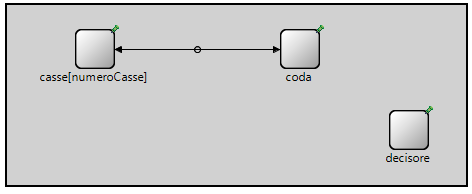
\includegraphics[width=90mm]{scenario.png}
  \caption{Generic scenario.}
  \label{fig:gs}
  \end{center}
\end{figure}
The model we thought generalizes both types of tails. The generic scenario is illustrated in \ref{fig:gs}:In this scheme, the customer, that is arrived, follows the workflow, from the input it’s inserted in the queue, the module D as “decisore” chooses using different policies to which till address the customer. At last, after the service time, the customer leaves the system. 
